\documentclass[letterpaper, 9pt]{extarticle}
% \usepackage{fontspec}

% ==================================================

% document parameters
% \usepackage[spanish, mexico, es-lcroman]{babel}
\usepackage[english]{babel}
\usepackage[margin=2cm]{geometry}

% ==================================================

% Packages for math
\usepackage{mathrsfs}
\usepackage{amsfonts}
\usepackage{amsmath}
\usepackage{amsthm}
\usepackage{amssymb}
\usepackage{physics}
\usepackage{dsfont}
\usepackage{esint}

% ==================================================

% Packages for writing
\usepackage{enumerate}
\usepackage[shortlabels]{enumitem}
\usepackage{framed}
\usepackage{csquotes}
\usepackage{gensymb}

% ==================================================

% Miscellaneous packages
\usepackage{float}
\usepackage{tabularx}
\usepackage{xcolor}
\usepackage{multicol}
\usepackage{subcaption}
\usepackage{caption}
\usepackage{graphicx}
\usepackage{array}
\usepackage{circuitikz}
\captionsetup{format = hang, margin = 10pt, font = small, labelfont = bf}
\usepackage{pgfplots} 

% Citation
\usepackage[round, authoryear]{natbib}

% Hyperlinks setup
\usepackage{hyperref}
\definecolor{links}{rgb}{0.36,0.54,0.66}
\hypersetup{
   colorlinks = true,
    linkcolor = black,
     urlcolor = blue,
    citecolor = blue,
    filecolor = blue,
    pdfauthor = {Author},
     pdftitle = {Title},
   pdfsubject = {subject},
  pdfkeywords = {one, two},
  pdfproducer = {LaTeX},
   pdfcreator = {pdfLaTeX},
   }

\usepackage{titlesec}
\usepackage[many]{tcolorbox}

% Adjust spacing after the chapter title
\titlespacing*{\chapter}{0cm}{-2.0cm}{0.50cm}
\titlespacing*{\section}{0cm}{0.50cm}{0.25cm}

% Indent 
\setlength{\parindent}{0pt}
\setlength{\parskip}{1ex}

% --- Theorems, lemma, corollary, postulate, definition ---
% \numberwithin{equation}{section}

\newtcbtheorem[]{problem}{Problem}%
    {enhanced,
    colback = black!5, %white,
    colbacktitle = black!5,
    coltitle = black,
    boxrule = 0pt,
    frame hidden,
    borderline west = {0.5mm}{0.0mm}{black},
    fonttitle = \bfseries\sffamily,
    breakable,
    before skip = 3ex,
    after skip = 3ex
}{problem}

\tcbuselibrary{skins, breakable}

% --- You can define your own color box. Just copy the previous \newtcbtheorm definition and use the colors of yout liking and the title you want to use.
% --- Basic commands ---
%   Euler's constant
\newcommand{\eu}{\mathrm{e}}

%   Imaginary unit
\newcommand{\im}{\mathrm{i}}

%   Sexagesimal degree symbol
\newcommand{\grado}{\,^{\circ}}

% --- Comandos para álgebra lineal ---
% Matrix transpose
\newcommand{\transpose}[1]{{#1}^{\mathsf{T}}}

%%% Comandos para cálculo
%   Definite integral from -\infty to +\infty
\newcommand{\Int}{\int\limits_{-\infty}^{\infty}}

%   Indefinite integral
\newcommand{\rint}[2]{\int{#1}\dd{#2}}

%  Definite integral
\newcommand{\Rint}[4]{\int\limits_{#1}^{#2}{#3}\dd{#4}}

%   Dot product symbol (use the command \bigcdot)
\makeatletter
\newcommand*\bigcdot{\mathpalette\bigcdot@{.5}}
\newcommand*\bigcdot@[2]{\mathbin{\vcenter{\hbox{\scalebox{#2}{$\m@th#1\bullet$}}}}}
\makeatother

%   Hamiltonian
\newcommand{\Ham}{\hat{\mathcal{H}}}

%   Trace
\renewcommand{\Tr}{\mathrm{Tr}}

% Christoffel symbol of the second kind
\newcommand{\christoffelsecond}[4]{\dfrac{1}{2}g^{#3 #4}(\partial_{#1} g_{#2 #4} + \partial_{#2} g_{#1 #4} - \partial_{#4} g_{#1 #2})}

% Riemann curvature tensor
\newcommand{\riemanncurvature}[5]{\partial_{#3} \Gamma_{#4 #2}^{#1} - \partial_{#4} \Gamma_{#3 #2}^{#1} + \Gamma_{#3 #5}^{#1} \Gamma_{#4 #2}^{#5} - \Gamma_{#4 #5}^{#1} \Gamma_{#3 #2}^{#5}}

% Covariant Riemann curvature tensor
\newcommand{\covariantriemanncurvature}[5]{g_{#1 #5} R^{#5}{}_{#2 #3 #4}}

% Ricci tensor
\newcommand{\riccitensor}[5]{g_{#1 #5} R^{#5}{}_{#2 #3 #4}}
\begin{document}
\setlist{itemsep=.5em}
\begin{Huge}
\textsf{\textbf{Fisica 2 (Teoria dei Circuiti)}}\\
Esperienza 1
\end{Huge}

\vspace{1ex}

\textsf{\textbf{Studenti:}} \text{Angelo Perotti},  \text{Mattia Zagatti}, \text{Mattia Dolci}

\vspace{2ex}

\section{Introduzione}

Lo scopo di questa esperienza di laboratorio è stato mettere in pratica le nozioni apprese durante le lezioni teoriche, osservando concretamente il comportamento dei circuiti studiati e delle strumentazioni. In particolare, abbiamo verificato la legge di Ohm, le leggi di Kirchhoff e il teorema di Millman. Durante l’esperienza abbiamo anche acquisito familiarità con l’utilizzo della strumentazione di base, come l’alimentatore e il multimetro, necessarie per eseguire misurazioni accurate e analizzare i circuiti.

\section{Materiale Utilizzato}
Di seguito è riportato il materiale necessario per l’esperimento:
\begin{itemize}
    \item \textbf{Componenti elettronici}: resistori (\(1 \, \text{k}\Omega\), \(10 \, \text{k}\Omega\), \(100 \, \text{k}\Omega\), \(1 \, \text{M}\Omega\), \(10 \, \text{M}\Omega\)), breadboard.
    \item \textbf{Strumenti di misura}: multimetro digitale, alimentatore da banco.
    \item \textbf{Cavi}: cavi banana-banana, cavi jumper.
\end{itemize}

\section{Cenni Teorici}

\begin{itemize}
    \item \textbf{Legge di Ohm}: \( V = R \cdot I \), che rappresenta la relazione caratteristica dei resistori.
    \item \textbf{Prima legge di Kirchhoff delle correnti}: \(\sum_{e=1}^{n} i_e = \sum_{u=1}^{m} i_u\), ovvero la somma delle correnti entranti in un nodo è uguale alla somma delle correnti uscenti.
    \item \textbf{Legge di Kirchhoff delle tensioni}: \(\sum_{k=1}^{n} V_k = 0\), ossia la somma algebrica delle tensioni in una maglia è nulla.
    \item \textbf{Teorema di Millman}: \( V_0 = \frac{\sum_{k=1}^{n} \frac{V_k}{R_k}}{\sum_{k=1}^{n} \frac{1}{R_k}} \), ovvero la tensione ai terminali di un nodo comune a \( n \) rami è il rapporto tra la somma delle tensioni divise per le rispettive resistenze e la somma dei reciproci delle resistenze.
\end{itemize}
\section{Esperimento 1: misura di tensione}

\subsection{Procedura Sperimentale}

È stato realizzato un partitore di tensione su breadboard (Figura 1), con un generatore da \(6 \, \text{V}\), due resistori in serie e un multimetro in parallelo al secondo resistore. Impostati i limiti di corrente e tensione del generatore a \(6 \, \text{mA}\) e \(6 \, \text{V}\), si è attivato il generatore e misurata la tensione ai capi del secondo resistore. Successivamente, si è variata la coppia di resistori per ogni misurazione.

\begin{figure}[h!] % Ambiente figure per centrare e aggiungere didascalia
    \centering % Centra l'immagine
    \begin{circuitikz}
        % Disegna la sorgente di tensione Vs
        \draw
        (0,0) to[battery, l_=$V_s$] (0,3)
        % Resistenza R1
        -- (2,3) to[R=$R_1$] (4,3)
        % Punto di giunzione tra R1 e R2
        -- (4,1.5) to[R=$R_2$] (4,0)
        % Collegamento alla massa (ground)
        -- (0,0)
        % Voltmetro in parallelo a R2
        (4,1.5) -- (5.5,1.5) to[voltmeter, l=$V$] (5.5,0) -- (4,0);
    \end{circuitikz}
    \caption{Circuito partitore di tensione.}
\end{figure}
\newpage
\subsection{Risultati}

La tabella seguente riporta i valori di tensione misurati e il confronto con i valori teorici per diverse configurazioni di \( R_1 \) e \( R_2 \):

\begin{center}
\begin{tabular}{ c | c | c | c | c}

Test & $R_1$ & $R_2$ & $V_{R_2}$ (misurato) & V$_{expected}$ \\ 
\hline
1 & \(1 \, \text{k}\Omega\) & \(1 \, \text{k}\Omega\) & 2.99 V & 3V\\ 
\hline
2 & \(1 \, \text{k}\Omega\) & \(500 \, \Omega\) & 1.99 V & 2V\\
\hline
3 & \(10 \, \text{k}\Omega\) & \(10 \, \text{k}\Omega\) & 2.99 V & 3V\\
\hline
4 & \(100 \, \text{k}\Omega\) & \(100 \, \text{k}\Omega\) & 2.98 V & 3V\\
\hline
5 & \(1 \, \text{M}\Omega\) & \(1 \, \text{M}\Omega\) & 2.84 V & 3V\\
\hline
6 & \(10 \, \text{M}\Omega\) & \(10 \, \text{M}\Omega\) & 1.84 V & 3V\\

\end{tabular}
\end{center}

\subsection{Analisi e Discussione} 
I risultati delle misurazioni mostrano una buona corrispondenza con i valori teorici per configurazioni di resistenze con valori bassi e medi. Tuttavia, quando vengono utilizzate resistenze elevate (nell’ordine dei megaohm), si osserva che la tensione misurata è inferiore rispetto al valore previsto teoricamente.

Questa discrepanza è attribuibile alla resistenza interna del multimetro, che si comporta come un carico addizionale nel circuito. La resistenza interna del multimetro è infatti confrontabile con i valori elevati dei resistori utilizzati in questi casi, introducendo un effetto di divisione di tensione non trascurabile.

Considerando una resistenza interna stimata nell’ordine di diversi megaohm, è possibile spiegare la diminuzione della tensione misurata ai capi del secondo resistore. Questo fenomeno evidenzia l’importanza di considerare le specifiche tecniche degli strumenti di misura, in particolare per configurazioni con elevati valori resistivi.

\subsection{Conclusione}
La verifica del partitore di tensione ha confermato la validità della teoria, mostrando una corrispondenza tra i valori teorici e quelli misurati per resistenze basse e medie. Tuttavia, per valori resistivi elevati (nell’ordine dei megaohm), la tensione misurata ha mostrato una deviazione dai valori teorici. Ciò è stato attribuito alla resistenza interna del multimetro, che ha introdotto un carico addizionale sul circuito. 

\section{Esperimento 2: teorema di Millman}
\subsection{Procedura Sperimentale}
\begin{figure}[h]
\begin{minipage}[t]{0.5\textwidth} % Regola la larghezza del minipage per il testo
\vspace{0pt}
    \raggedright % Allinea a sinistra
    Nella seconda parte di questa esperienza di laboratorio è stato illustrato il teorema di Millman, derivato dalle leggi di Kirchhoff, che permette di calcolare la tensione ai capi di un nodo comune ad $n$ rami con generatori di tensione e resistenze in parallelo. Il teorema è stato poi verificato sperimentalmente costruendo il circuito mostrato in Figure 2.\\
    \vspace{0.05\textwidth}
    Il circuito è stato realizzato con tre generatori di tensione connessi ciascuno in serie a un resistore da $1 \, \text{k}\Omega$, e una resistenza da $10 \, \text{k}\Omega$ collegata in parallelo ai tre rami. Il multimetro, configurato come amperometro, è stato usato per misurare la corrente nei rami con i generatori, e successivamente è stata misurata la tensione ai capi della resistenza da $10 \, \text{k}\Omega$. I risultati delle misurazioni sono riportati nella seguente tabella.
\end{minipage}%
\hspace{0.05\textwidth} % Spazio tra il testo e l'immagine
\begin{minipage}[t]{0.4\textwidth} % Regola la larghezza del minipage per l'immagine
\vspace{0pt}
    \centering
    \resizebox{1.2\textwidth}{!}{%
\begin{circuitikz}
\tikzstyle{every node}=[font=\LARGE]
\draw (8.75,14.75) to[battery1] (8.75,17.25);
\draw (6.25,17.25) to[battery1] (6.25,14.75);
\draw (3.75,17.25) to[battery1] (3.75,14.75);
\draw (3.75,17.25) to[R] (3.75,19.75);
\draw (6.25,17.25) to[R] (6.25,19.75);
\draw (8.75,17.25) to[R] (8.75,19.75);
\draw (3.75,19.75) to[rmeter, t=A] (3.75,21);
\draw (6.25,19.75) to[rmeter, t=A] (6.25,21);
\draw (8.75,19.75) to[rmeter, t=A] (8.75,21);
\draw (3.75,21) to[short] (8.75,21);
\draw (3.75,14.75) to[short] (8.75,14.75);
\draw (8.75,14.75) to[short] (11.25,14.75);
\draw (11.25,16) to[R] (11.25,18.5);
\draw (11.25,14.75) to[short] (11.25,16);
\draw (11.25,16) to[short] (13.75,16);
\draw (13.75,18.5) to[short] (11.25,18.5);
\draw (11.25,18.5) to[short] (11.25,21);
\draw (11.25,21) to[short] (8.75,21);
\draw (13.75,18.5) to[rmeter, t=V] (13.75,16);
\draw (7.5,14.75) to (7.5,13.5) node[sground]{};
\node [font=\LARGE] at (2.5,18.25) {1K$\Omega$};
\node [font=\LARGE] at (2.5,16.25) {8V};
\node [font=\LARGE] at (5,16.25) {5V};
\node [font=\LARGE] at (5,18.25) {1K$\Omega$};
\node [font=\LARGE] at (7.5,18.25) {1K$\Omega$};
\node [font=\LARGE] at (7.5,16.25) {3V};
\node [font=\LARGE] at (10,17.25) {10K$\Omega$};
\end{circuitikz}
}%
    \caption{Circuito utilizzato per l'esperimento.}
    \label{fig:circuito}
\end{minipage}
\end{figure}


\subsection{Risultati}
\begin{center}
        \begin{tabular}{c|c|c}
        Ramo misurato &  Tensione & Corrente\\
        \hline
         1 Ramo & +8V & +1,7mA \\
    \hline
         2 Ramo & +5V & +4,7mA \\
    \hline
         3 Ramo & -3V & -6,05mA
    \end{tabular}
\end{center}

\subsection{Analisi e Discussione}
Applichiamo Millman utilizzando i risultati ottenuti sperimentalmente:
\begin{center}
    \resizebox{0.6\textwidth}{!}{
    $V_0=\dfrac{\sum_i\dfrac{V_c}{R_c}}{\sum_i\dfrac{1}{R_i}}=\dfrac{\dfrac{8V}{1K\Omega}+\dfrac{5V}{1K\Omega}-\dfrac{3V}{1K\Omega}}{\dfrac{1}{1K\Omega}+\dfrac{1}{1K\Omega}+\dfrac{1}{1K\Omega}+\dfrac{1}{10K\Omega}}=\dfrac{\dfrac{10V}{1K\Omega}}{\dfrac{31}{10K\Omega}}=\dfrac{10V \cdot 10K\Omega}{1K\Omega \cdot 31}= 3,22V$}
\end{center}
È possibile notare che la tensione misurata ai capi del resistore da $10 \, \text{k}\Omega$ risulta vicina al valore teorico calcolato con il teorema di Millman, confermandone la validità.\\
Possiamo ora stimare la corrente di lato sul resistore da \(10 \, \text{k}\Omega\) applicando la legge di Kirchhoff ai nodi: 
\[
I_1 + I_2 + I_3 + I_{10\text{k}\Omega} = 0
\]
Con \(I_1\), \(I_2\) e \(I_3\) le correnti misurate rispettivamente nei tre rami e \(I_{10\text{k}\Omega}\) la corrente di lato nel resistore da \(10 \, \text{k}\Omega\), da cui:
\[
I_{10\text{k}\Omega} = -(1.7 \, \text{mA} + 4.7 \, \text{mA} - 6.05 \, \text{mA}) \longrightarrow I_{10\text{k}\Omega} = -0.35 \, \text{mA}
\]



Pertanto, la corrente di lato attraverso il resistore da \(10 \, \text{k}\Omega\) è: $I_{10\text{k}\Omega} = 0.35 \, \text{mA}$


Questa corrente conferma il bilancio delle correnti nel nodo e rispetta la legge di Kirchhoff.

\subsection{Conclusione}
L’esperimento ha dimostrato la validità del Teorema di Millman, con la tensione calcolata teoricamente corrispondente ai valori sperimentali misurati. L’applicazione delle leggi di Kirchhoff ha inoltre confermato il bilancio delle correnti nel nodo, validando ulteriormente i principi teorici. La capacità di calcolare tensioni e correnti nei circuiti complessi è stata consolidata attraverso la verifica pratica del teorema.

\section{Esperimento 3: Legge di Ohm}
\subsection{Procedura Sperimentale}
Lo scopo dell’esercizio è quello di misurare il rapporto corrente/tensione riguardo al circuito in Figura 3, composto da un resistore da $500\Omega$ e da una tensione di Vs che assume valori diversi, i risultati delle misurazioni sono riportati in tabella.
\begin{figure}[h]
\begin{minipage}[t]{0.5\textwidth} % Regola la larghezza del minipage per il testo
\vspace{0pt}
    \raggedright % Allinea a sinistra
    La tensione Vs viene generata da un alimentatore, mentre la corrente viene misurata mediante un multimetro configurato come amperometro, posizionato in serie al resistore. 
\end{minipage}%
\hspace{0.05\textwidth} % Spazio tra il testo e l'immagine
\begin{minipage}[t]{0.15\textwidth} % Regola la larghezza del minipage per l'immagine
\vspace{0pt}
    \centering
    \resizebox{1\textwidth}{!}{%
\begin{center}
    \begin{circuitikz}
\tikzstyle{every node}=[font=\LARGE]
\draw (8.75,18.5) to[battery1] (8.75,16);
\draw (8.75,18.5) to[rmeter, t=A] (12.5,18.5);
\draw (12.5,18.5) to[R] (12.5,16);
\draw (8.75,16) to[short] (12.5,16);
\draw (10.75,16) to (10.75,15.5) node[sground]{};
\node [font=\LARGE] at (7.75,17.25) {$V_S$};
\node [font=\LARGE] at (11.75,17.25) {$R_1$};
\end{circuitikz}
\end{center}
   
}%
    \caption{}
    \label{fig:circuito}
\end{minipage}
\end{figure} 
\newpage

\subsection{Risultati}
\begin{figure}[ht]
    \centering
    \begin{minipage}{0.35\textwidth}
        \centering
        \begin{tabular}{c|c|c|c|c}
            \toprule
            $V_s$ [V] & $I_s$ [mA] & $I_t$ [mA] & ${I_s}/{V_s}$ &I_t/V\\
            \hline
            \midrule
            1    & 2.02  & 2    & 2.02  & 2\\
            \hline
            2    & 4.04  & 4    & 2.02  & 2\\
            \hline
            3    & 6.07  & 6    & 2.02  & 2\\
            \hline

            4    & 8.08  & 8    & 2.02  & 2\\
            \hline

            5    & 10.1  & 10   & 2.02  & 2\\
            \hline

            6    & 12.1  & 12   & 2.02  & 2\\
            \hline

            7    & 14.1  & 14   & 2.02  & 2\\
            \hline

            8    & 16.2  & 16   & 2.02  & 2\\
            \bottomrule
        \end{tabular}
    \end{minipage}%
    \hspace{0.05\textwidth}
    \begin{minipage}{0.59\textwidth}
        \centering
        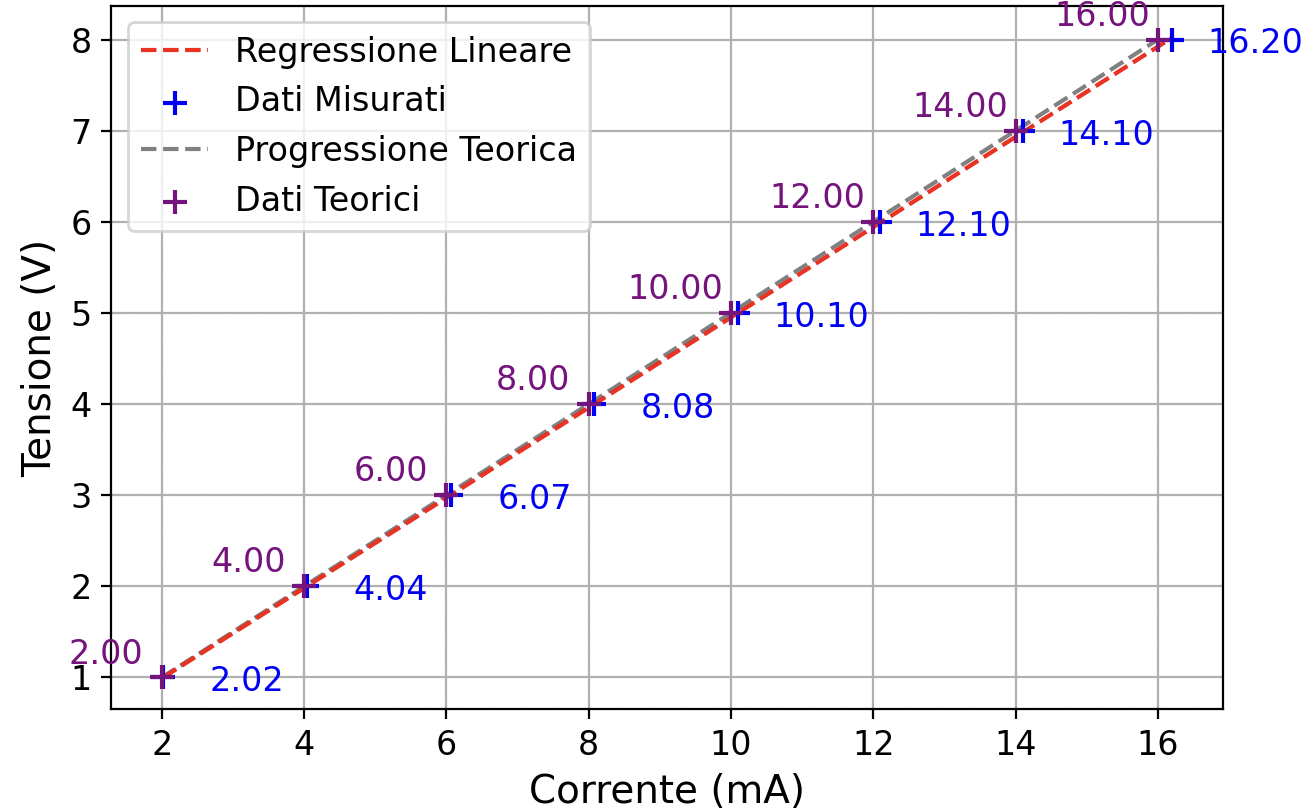
\includegraphics[width=\linewidth]{immagine1.png}
        \caption{Grafico corrente-tensione con regressione lineare sui dati}
        \label{fig:immagine}
    \end{minipage}
\end{figure}
\subsection{Analisi e Discussione}
L’esperimento si è basato sull’applicazione della Legge di Ohm, che stabilisce che la corrente  I  che attraversa un resistore è direttamente proporzionale alla tensione  V  applicata ai suoi capi e inversamente proporzionale alla resistenza  R  del componente:
$I = \frac{V}{R}$

Questa relazione implica che, in un circuito lineare, il rapporto $\frac{V}{I}$ rimane costante ed è pari alla resistenza del resistore, mentre il reciproco di tale valore è noto come conduttanza ( G ), misurata in Siemens.

Durante l’esperimento, sono stati raccolti valori di corrente misurati ( $I_s$ ) e teorici ( $I_t$ ), confrontando questi ultimi con i valori calcolati dalla relazione  $I_t = \frac{V_s}{R}$. I risultati dimostrano che il rapporto tra tensione e corrente si mantiene costante, con lievi discrepanze tra i valori misurati e teorici, ottenuti applicando la legge di Ohm.
Vediamo come, applicando la legge in questione, il rapporto tra corrente e tensione risulta sempre circa uguale a 2, questo perché esse sono legate da un rapporto di proporzionalità diretta. Il valore ricavato è chiamato conduttanza, si misura in siemens ed esprime l’attitudine di un conduttore ad essere percorso da corrente elettrica.

\subsection{Conclusione}
L’analisi del circuito resistivo ha confermato che il rapporto tra corrente e tensione è costante, come previsto dalla Legge di Ohm. Il valore sperimentale della conduttanza è risultato prossimo a quello teorico, con leggere discrepanze attribuibili alla tolleranza del resistore utilizzato. La relazione lineare tra tensione e corrente, evidenziata anche graficamente, ha fornito un riscontro chiaro della proporzionalità diretta descritta dalla legge.

%\section{Conclusioni}
%bo figata lo rifarei solo per sentire le storie di contrabbando del daddy proibito
\end{document}